\cleardoublepage

\newrefsection

\chapter{外文翻译}

由于原文翻译比较长,这里仅仅截取其摘要、设计以及测试分析的部分。

\sectionnonum{摘要}

发现内核并发错误通过模糊测试是具有挑战性的。识别内核并发错误,与非并发错误相反,需要分析两个或多个线程之间可能的交错情况。然而,由于线程交错的搜索空间非常庞大,因此不可能调查所有可能的线程交错情况是不切实际的。为了探索这个庞大的搜索空间,大多数先前的方法执行随机或简单的启发式搜索,而没有线程交错的覆盖,或者覆盖形式不足够。结果,它们要么进行了浪费执行的无用搜索,要么忽视了其覆盖范围无法解决的并发错误。为了克服这些限制,我们提出了SEGFUZZ,这是一个用于内核并发错误的模糊测试框架。在探索线程交错的搜索空间时,SEGFUZZ将整个线程交错分解为一组段,每个段代表少量指令的交错,并将各个段用作交错覆盖,称为交错段覆盖。在搜索线程交错时,SEGFUZZ会变异已探索的交错段中的交错,以构建尚未探索的新线程交错。通过SEGFUZZ,我们在Linux内核中发现了21个新的并发错误,并通过展示SEGFUZZ可以比现有技术平均快4.1倍地识别已知错误来展示SEGFUZZ的效率。

\section{SEGFUZZ的设计}

SEGFUZZ是一种采用了交错段覆盖和基于突变的交错的探索的内核并发模糊器。如\autoref{fig:fig5}所示,SEGFUZZ包含两个阶段的模糊测试。 第一阶段是单线程的模糊测试,使用分支覆盖来搜索执行路径,第二阶段是多线程模糊测试,使用交错段覆盖来探索线程交错。在两个阶段中,SEGFUZZ都会跟踪每个系统调用下面执行的带有时间戳注释的内存访问,第二阶段还会采用一种控制线程调度的机制。
    
接下来,我们提供了SEGFUZZ的整体设计。然后,我们描述了用于跟踪带时间戳注释的内存访问的内核工具,以及控制线程调度的执行引擎。最后,我们将解释SEGFUZZ的实现细节。

\begin{figure}[ht]
    \centering
    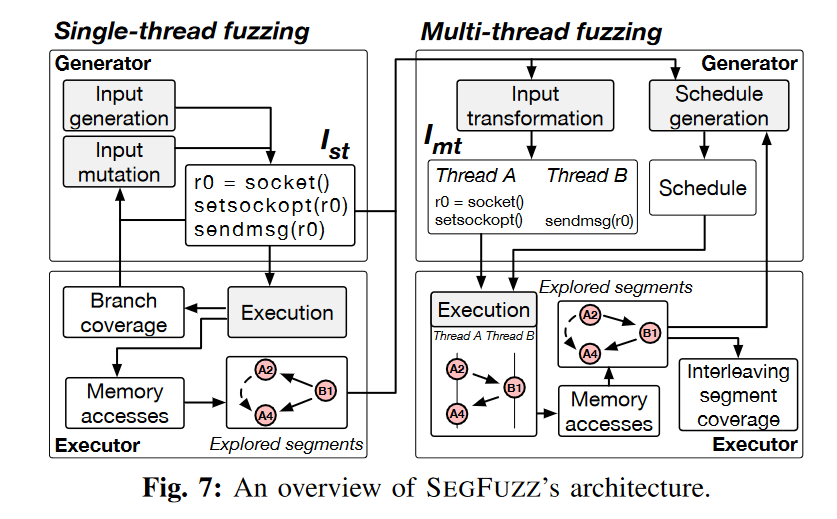
\includegraphics[width=0.8\linewidth]{fig5}
    \caption{\label{fig:fig5}SEGFUZZ架构概述}
\end{figure}

\subsection{两阶段模糊测试}

SERFUZZ的单线程模糊测试和多线程模糊测试均由两个部分组成,分别是一个输入生成器和一个输入执行器。我们将在后面解释每一个细节。

\subsubsection{单线程模糊测试}

在单线程模糊测试阶段,单线程生成器以随机系统调用序列(S1, S2, ... )的形式产生单线程输入(称为$I_{ST}$)。然后,单线程执行器通过运行$I_{ST}$来识别可能会导致新的交错覆盖段的两个系统调用。如果确定,$I_{ST}$将被传递到下一阶段,即多线程模糊测试。

\paragraph{单线程生成器}与传统的模糊测试类似,单线程生成器使用生成和变异两种策略构造单线程的输入$I_{ST}$。当使用生成策略时,SEGFUZZ基于格式良好的系统调用描述语法Syzlang随机生成系统调用序列。这个序列描述了可用系统调用的模板,包括参数类型、每个参数的可能值范围以及返回值的类型。使用Syzlang,SEGFUZZ通过重复选择随机系统调用并提供系统调用的可能的参数来生成单线程输入。突变策略是生成策略的替代方案。使用突变策略时,SEGFUZZ会选取已生成的单线程输入,并通过添加系统调用、删除现有系统调用或更改现有系统调用的参数值来修改单线程输入。

单线程执行器。给定来自单线程生成器的$I_{ST}$,单线程执行器运行$I_{ST}$,同时跟踪每个系统调用所执行的基本块和带时间戳注释的内存访问。执行完成后,单线程执行器计算分支覆盖率,如果$I_{ST}$暴露了尚未探索的新分支覆盖率, SEGFUZZ就保留这个$I_{ST}$ ,并将其反馈给单线程生成器,以便单线程生成器进一步改变$I_{ST}$找到更多的分支覆盖范围。
此外,单线程执行器识别$I_{ST}$中的一对系统调用,如果同时执行,它们可能会暴露新的交错段覆盖。具体来说,对于$I_{ST}$中的每个系统调用对$(S_i , S_j)$,单线程执行器计算一组探索段图G ,其中$S_i$和$S_j$执行访问的内存(如第 IV‑B 节所述),并检查G是否包含尚未探索的新段图。如果是,单线程执行器将$I_{ST}$以及$(S_i , S_j)$和G传递给多线程模糊测试。多线程模糊测试将$I_{ST}$分成两个系统调用序列,目的是同时运行$S_i$和$S_j$。

单线程模糊测试中的 CVE-2017-17712。为了发现图1中演示的 CVE-2017-17712 ,我们假设单线程生成器将$I_{ST}$生成为三个系统调用序列r0 = socket()、setsocktopt(r0)、 sendmsg(r0),如图7中所述。然后,单线程执行器运行这个$I_{ST}$ ,并收集两个系统调用setsockopt(r0)和sendmsg(r0) 执行的内存访问。由于这些内存访问都带有时间戳注释,单线程执行器可以识别出setsockopt(r0)执行的所有内存访问后面都是sendmsg(r0)执行的内存访问,并计算一组段图G,其中包括($B1 \Rightarrow A2 \Rightarrow A4$) (即\autoref{fig:fig6}‑(a))。假设之前没有见过($B1 \Rightarrow A2 \Rightarrow A4$),SEGFUZZ将会确定值得探索两个系统调用之间的交错。因此,单线程执行器将$I_{ST}$以及两个系统调用和G传递到下一个阶段。

\begin{figure}[ht]
    \centering
    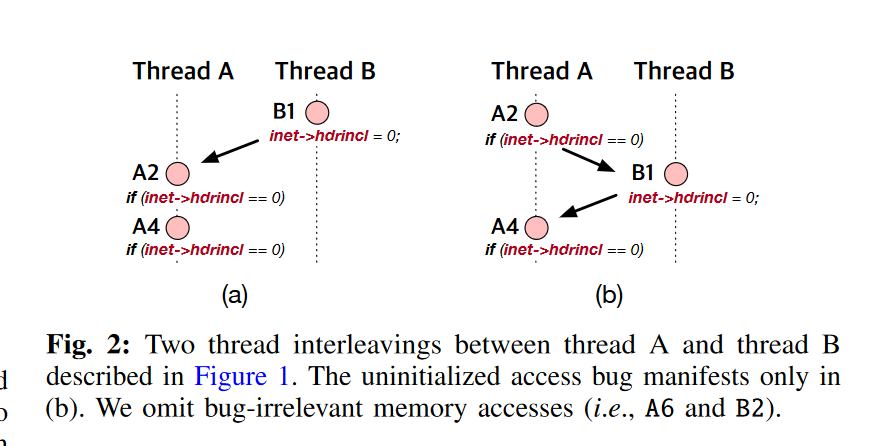
\includegraphics[width=0.8\linewidth]{fig6}
    \caption{\label{fig:fig6}图1中描述的线程 A 和线程 B 之间的两个线程交错。未初始化的访问错误仅出现在(b) 中。我们省略了与 bug 无关的内存访问(即 A6 和 B2)。}
\end{figure}

\subsubsection{多线程模糊测试}

在$I_{ST}$与$(S_i, S_j)$和G被一起传递多线程生成器后,多线程生成器将$I_{ST}$转换为多线程输入$I_{MT}$。此外,多线程生成器根据基于突变的交错探索(§IV-C)生成调度。然后,多线程执行器在执行引擎(§V-C)的支持下测试$I_{MT}$的每个调度,并收集交错段覆盖率(§IV-B)。
    
\paragraph{多线程生成器}给定$I_{ST}$和$(S_i, S_j)$,多线程生成器首先生成$I_{MT}$ ,它保留$I_{ST}$中的所有系统调用,但同时执行$S_i$和$S_j$ 。具体来说,假设i < j,多线程生成器分割$I_{ST}$ ,它将系统调用的单个序列(S1, S2, ..., , ..., $S_j$ , ..., Sn-1, Sn ),分为两个系统调用序列, ( S1, S2, ..., $S_i$)和($S_i$+1, ...$S_j$ ,..., Sn)。然后,多线程执行器在两个不同的线程中运行两个系统调用序列,同时运行$S_i$和$S_j$ 。附录C中提供了详细示例。

此外,多线程生成器重复产生各种调度。为了生成调度,多线程生成器实现第 IV-C 节中详细介绍的基于突变的交错探索方法。简单解释,给定一组已探索的线段图G,多线程生成器对G中的线段图进行变异,得到一组未探索的变异线段图Gmutated,然后选择Gmutated的一个子集G*来生成调度。多线程执行器发生变化,然后运行$I_{MT}$ ,同时强制执行生成的调度。
多线程执行器。多线程执行器运行$I_{MT}$ ,同时执行由多线程生成器生成的调度。在$I_{MT}$执行期间,多线程执行器在 lockdep、内核看门狗和 sanitizers 等开发者工具的支持下检查正在运行的线程交错是否会导致有害行为(例如内存损坏或死锁)。如果这些开发工具检测到内核中发生异常行为,多线程执行器会记录异常行为以及$I_{MT}$和执行的线程交错信息的报告。
否则,通过$S_i$和$S_j$执行的内存访问,多线程执行器计算一组执行的段图G’和关于交错段覆盖的探测,如第 IV-B节中所述。此外,多线程执行器将G’反馈到多线程生成器,允许多线程生成器进一步探索线程交错。
多线程模糊测试中的 CVE-2017-17712。一旦接收到$I_{ST}$ ,多线程生成器将$I_{ST}$转换为$I_{MT}$ 。在此示例中,线程 A 执行两个系统调用r0 = socket和setsockopt(r0),线程 B 执行一个系统调用sendmsg(r0),同时这两个系统调用setsockopt(r0)和sendmsg(r0)会被并发执行(如图7中的$I_{MT}$所示)。此外,多线程生成器根据基于突变的交错探索产生调度。给定$G(B1 \Rightarrow A2 \Rightarrow A4)$,多线程生成器会生成对应于$(A2 \Rightarrow B2 \Rightarrow A4)$的变异线段图(参见\autoref{fig:fig7})。然后,多线程生成器生成一个调度来测试$(A2\Rightarrow B1\Rightarrow A4)$ (参见\autoref{fig:fig8})。最后,当多线程执行器使用生成的调度运行$I_{MT}$时,会触发未初始化的访问错误

\begin{figure}[ht]
    \centering
    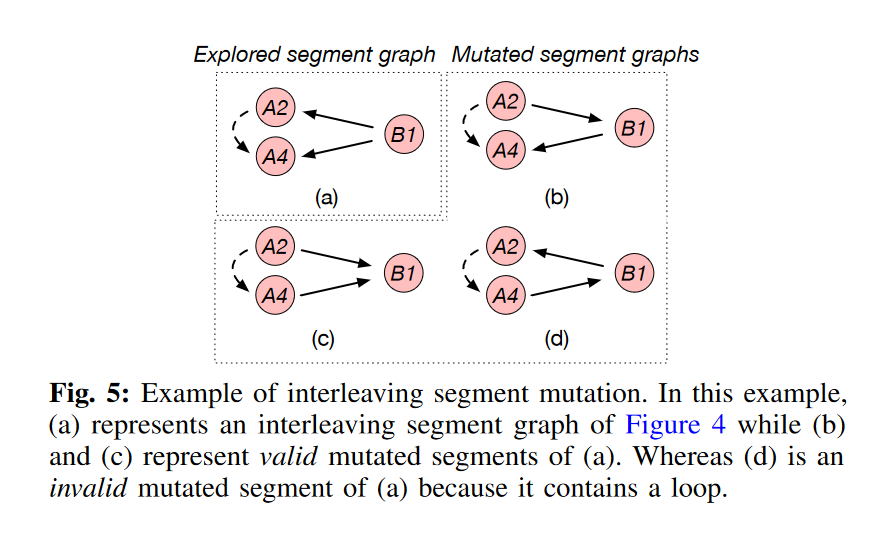
\includegraphics[width=0.8\linewidth]{fig7}
    \caption{\label{fig:fig7}交错片段突变的示例。在此示例中,(a) 表示\autoref{fig:fig6}的交错段图,而 (b) 和 (c) 表示 (a) 的有效变异段。而 (d) 是(a) 的无效变异片段,因为它包含循环。}
\end{figure}

\begin{figure}[ht]
    \centering
    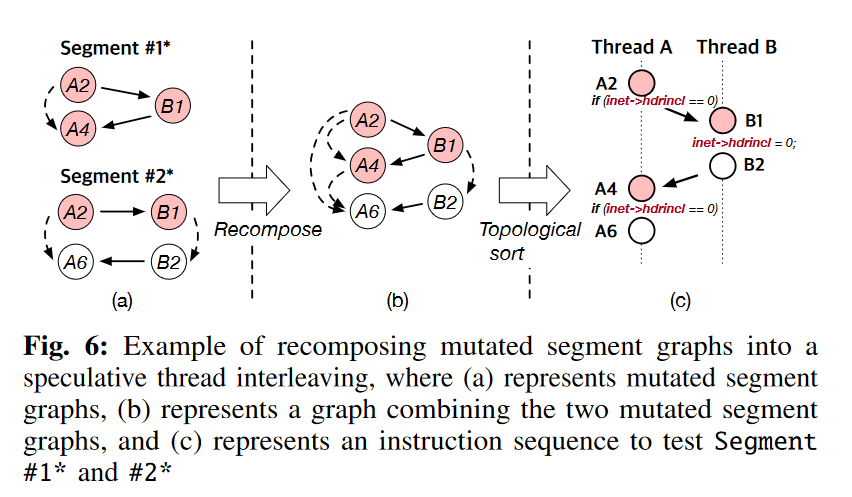
\includegraphics[width=0.8\linewidth]{fig8}
    \caption{\label{fig:fig8}将变异段图重新组合为推测线程交错的示例,其中(a) 表示变异段图,(b) 表示组合两个变异段图的图,(c) 表示测试段的指令序列 1 和 2}
\end{figure}

\subsection{内核检测}

SEGFUZZ需要跟踪每个系统调用执行的基本块(用于计算代码覆盖率)和带时间戳注释的内存访问(用于计算交错覆盖率)。为此,SEGFUZZ应用了一个编译器通道,该编译器通道在 1) 每个基本块的入口处以及 2) 访问全局可见内存对象的每条指令之前插入回调函数调用。在基本块的入口处,回调函数将基本块的起始地址记录到每线程内存区域中,该内存区域通过 mmap 在用户空间和内核空间之间共享。这样,线程执行系统调用后,可以通过读取内存区域来识别执行的基本块。与基本块的情况类似,在访问全局可见内存对象的指令上,回调函数记录了五个元组(即内存对象的地址、指令地址、内存访问的大小和类型、以及时间戳)。

\subsection{执行引擎}

执行引擎赋予模糊器进程控制线程调度的能力。它在虚拟机管理程序层中实现,不会干扰内核执行。

执行时间表。为了请求执行引擎强制执行计划,模糊器进程在执行系统调用之前通过超级调用接口发送计划。在运行期间,执行引擎按照给定时间表中的描述暂停和恢复系统调用的执行。

\autoref{fig:fig9}显示了执行引擎的工作流程。一开始,模糊器进程会生成线程,其中每个线程都被分配一个系统调用和调度点(\autoref{fig:fig9}中的1 )。然后,每个线程调用超级调用(即hcall\_sched())将调度点传递给执行引擎( 2 )。当执行引擎接收到调度点时,执行引擎在调度点所引用的指令上安装断点(2-1)。值得注意的是, hcall\_sched()将调度点的顺序作为第二个参数。本例中,执行过程中先抢占A2,然后依次抢占B2 、A6。交付调度点后,每个线程调用hcall\_ready(),该线程会休眠,直到所有线程调用就绪,所有线程调用hcall\_ready()后,执行引擎将它们唤醒,线程开始执行系统调用( 3 )。在执行系统调用时,执行引擎只保留一个线程执行。当正在运行的线程到达调度点时,执行引擎通过挂起正在运行的线程并恢复下一个线程按照给定调度(4-1)中指定的方式运行来抢占( 4 )。

\begin{figure}[ht]
    \centering
    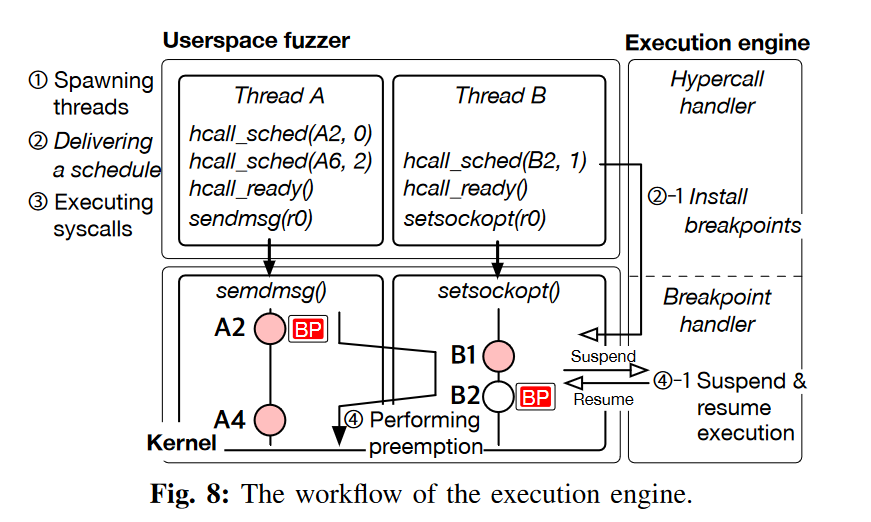
\includegraphics[width=0.8\linewidth]{fig9}
    \caption{\label{fig:fig9}执行引擎的工作流程}
\end{figure}

\paragraph{执行抢占}为了进行抢占, SEGFUZZ利用现代 Intel CPU 芯片组中提供的硬件断点功能。在抢占过程中,当遇到断点时,执行引擎会识别出运行已到达调度点。当线程遇到断点时,执行引擎将正在运行的线程的上下文信息(例如,寄存器值)存储在管理程序的存储器中,并将线程的程序计数器更改为称为蹦床的无限循环。在蹦床中,线程不断调用内核 API cond\_resched()来让出CPU。结果,线程被挂起在蹦床中而没有取得任何作用。为了恢复挂起的线程,执行引擎将寄存器(包括程序计数器)恢复为线程挂起时存储的值,然后线程可以继续运行。

\paragraph{硬件断点的限制}虽然SEGFUZZ通常需要四个以上的调度点,但可以同时安装的硬件断点的数量是有限的(例如,Intel CPU芯片组中为四个。SEGFUZZ通过利用调度点是有序的这一事实克服了这一限制。具体地,执行引擎在前四个调度点上设置断点,当命中已设置的断点时,执行引擎将断点移动到下一个调度点上。

\paragraph{处理缺失的调度点}在执行过程中,安装了调度点的指令可能不会被执行,例如,如果控制流由于内核内部状态而发生变化。在这种情况下,执行引擎不会打乱调度点的顺序。例如,当执行\autoref{fig:fig9}的调度时,线程 A 可能会跳过A2,并命中安装在 A6 上的断点。如果是,则执行引擎忽略A6之前的所有调度点(即A2和B2),并继续执行A6之后的调度。


\paragraph{虚拟机自省(VMI)}。执行引擎自省目标内核有两个原因。首先,由于断点不区分是哪个线程击中断点,因此执行引擎需要确定断点是由模糊器进程的线程击中,还是由不相关的线程击中。其次,当正在运行的线程尝试获取锁时,执行引擎会检查该锁是否已被挂起的线程持有,这可能会导致意外阻塞。虽然 VMI 对于正确控制线程调度至关重要,但我们将 VMI 的详细信息保留在附录D中。

\section{评估}

\subsection{寻找真实世界的并发漏洞}
\paragraph{新发现的并发错误}在我们的评估期间, SEGFUZZ发现了 83 个不同的崩溃,其中包括Syzkaller也发现的。其中21个新确定为有害并发错误,几个月后Syzkaller报告了3 个(即\#2、 \#3和\#5) 。结果总结在\autoref{fig:fig10}中。该结果表明, SEGFUZZ能够在整个内核层中找到从特定设备驱动程序(例如, \#1和\#3)到各种网络子系统(例如,\#8、\#12和\#21)。与专注于内核文件系统的KRACE不同, SEGFUZZ并非针对特定子系统定制。 SEGFUZZ不仅可以发现危害较小的错误,例如警告(例如,\#12,还可以发现严重的错误,例如内存损坏(例如,\#2、\#10和\#13)。有趣的是,根据内核开发人员对根本原因的确认,我们发现一些错误已经在内核中存在很长时间了,但从未被其他模糊测试系统识别出来。\#10 (即KASAN:slip\_ioctl 中的 use-after-freeRead)自 2013 年以来一直存在于内核中,而\#11 (即add\_wait\_queue 中的一般保护错误)自2011 年以来一直存在。这些案例表明SEGFUZZ能够发现很难发现并发错误。

\begin{figure}[ht]
    \centering
    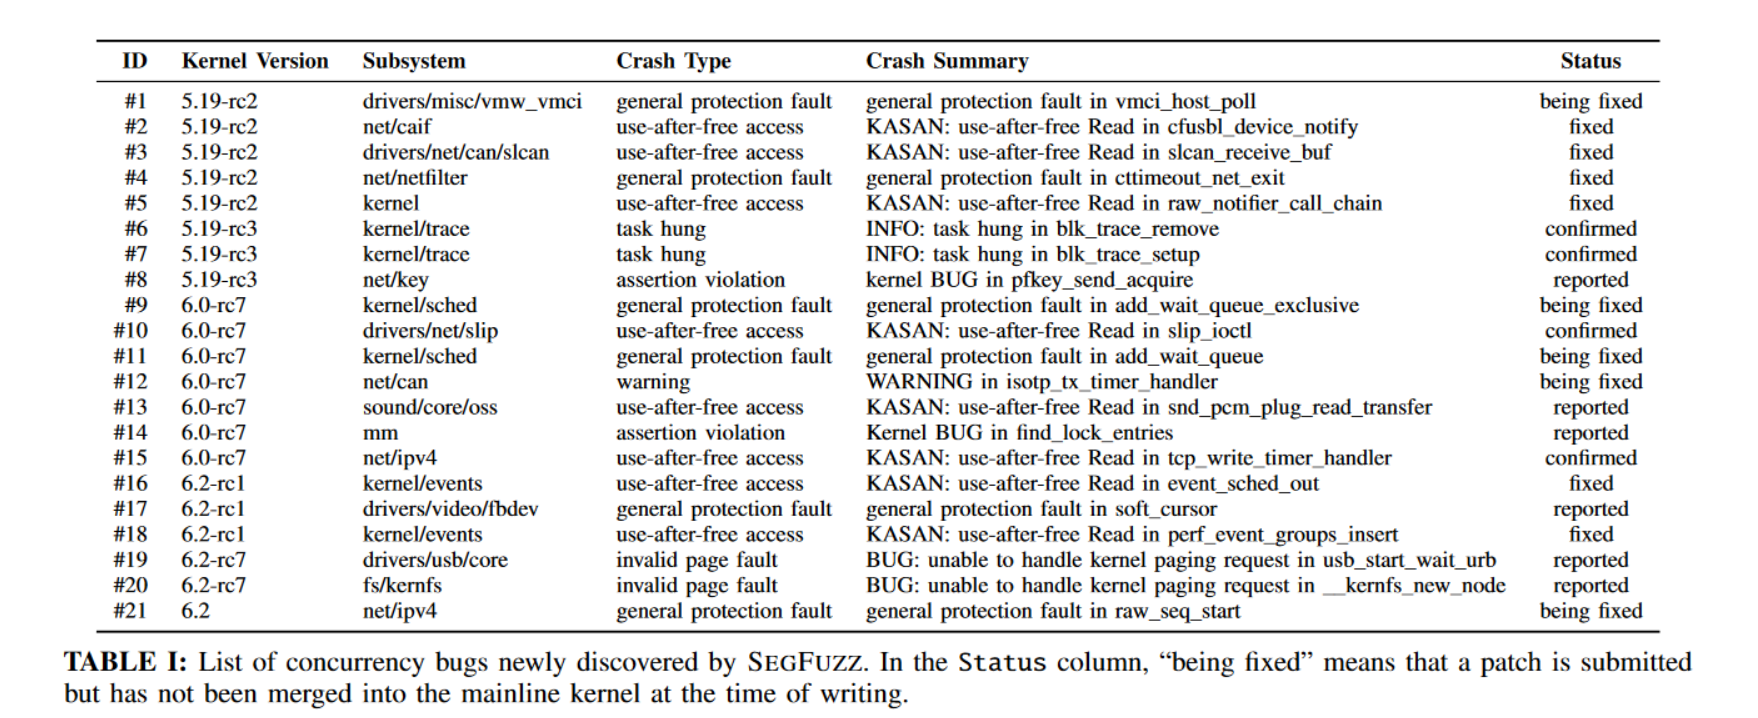
\includegraphics[width=0.8\linewidth]{fig10}
    \caption{\label{fig:fig10}SEGFUZZ新发现的并发错误列表。状态栏中“正在修复”表示补丁已提交,但在撰写本文时尚未合并到主线内核中。}
\end{figure}

\subsection{与之前的方法比较}

我们将SEGFUZZ与之前的方法进行比较,以回答以下问题:1)交错段覆盖(§IV-B)是否提供信息并有助于发现并发错误? (§III中的设计目标 1 ) (§VI-B1),以及 2)基于突变的交错探索(§IV-C)在探索线程交错的搜索空间方面的效率如何?(设计目标2) (§VI-B2)。为了评估这些点,我们收集了众所周知的并发错误作为测试集,然后在测试集上比较SEGFUZZ和之前的方法。

\paragraph{错误选择}\autoref{fig:fig11}显示了比较研究的并发错误。我们的并发错误选择标准是1)在之前的研究中研究了并发错误,2)我们可以找到修复并发错误的补丁,以便我们可以将它们注入内核。我们排除了ExpRace 中评估的两个Android 特定并发错误(即 CVE-2019-199和 CVE-2019-2025) 。为了在一致的环境上运行测试,我们使用相同的内核。

\begin{figure}[ht]
    \centering
    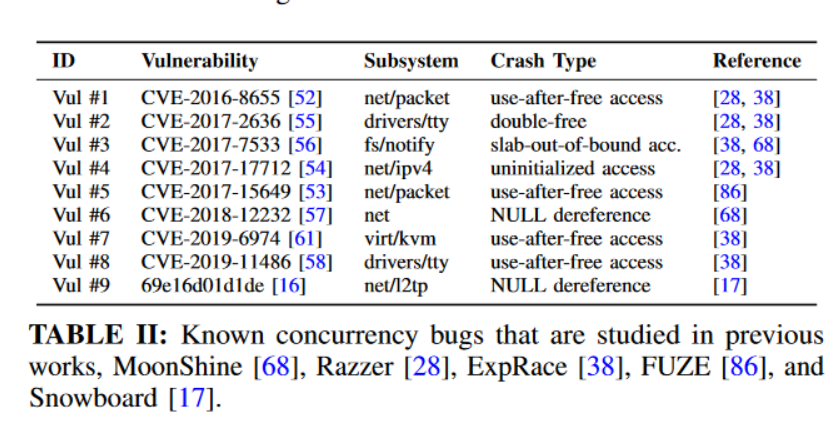
\includegraphics[width=0.8\linewidth]{fig11}
    \caption{\label{fig:fig11}之前研究的已知并发错误}
\end{figure}

\subsubsection{交错覆盖度量的比较}

我们在SEGFUZZ中实现了不同的覆盖度量并比较了使用交错段覆盖的SEGFUZZ版本。

\paragraph{比较目标}我们选择别名覆盖率作为比较目标,因为它是与以下内容最相关的交错覆盖率指标。然而,别名覆盖仅实现了对文件系统的检测,因此我们在SEGFUZZ中模拟别名覆盖,通过限制每个线段图的顶点数量到两个。因此,就像别名覆盖一样,交错段大小为2的包含两条指令之间的单个交错,其中至少有一个是写指令。使用模拟别名覆盖率,我们运行SEGFUZZ来查看每个并发错误是否被触发,直到模拟别名覆盖已饱和。
\paragraph{结果}表III显示了结果。 使用模拟别名覆盖率时,即使模拟别名覆盖率完全饱和,也不会发现许多(九个中的六个)并发错误。与使用交错段覆盖相比,SEGFUZZ 可以在每次试验中交错段覆盖饱和之前发现所有列出的并发错误。 第 III 节(即图 1)中描述的 CVE-2017-17712 示例解释了为什么会出现这样的结果; 模拟别名覆盖仅考虑两条指令之间的交错,这不足以执行包含多个指令的违规交错。我们手动识别出所有列出的并发错误都是由三个或四个指令的线程交错引起的,这支持我们对交错段大小的设计选择(§IV-A)。 另一方面,别名覆盖范围很快就饱和了。 通过我们基于突变的交错探索,平均执行 13.9 次(范围从 6 到 32 次)后就饱和了。

\begin{figure}[ht]
    \centering
    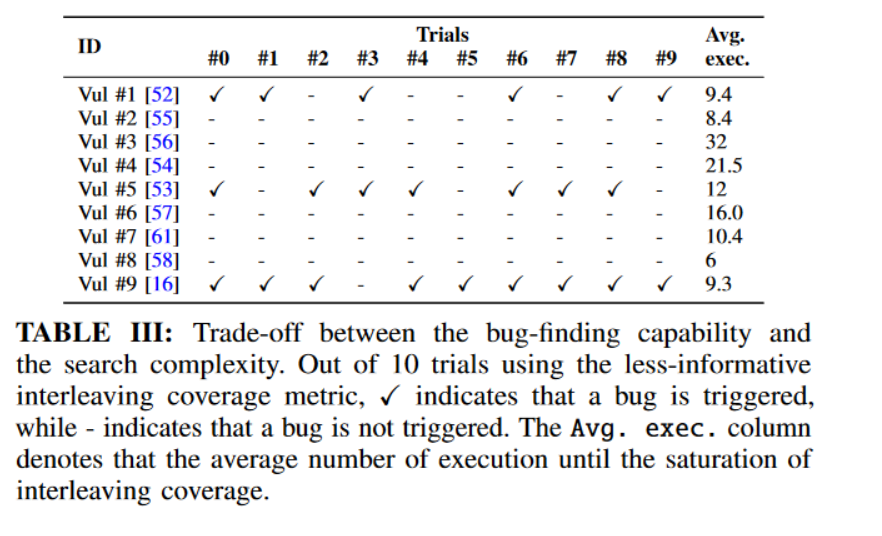
\includegraphics[width=0.8\linewidth]{fig12}
    \caption{\label{fig:fig12}错误查找能力和搜索复杂性之间的权衡。 在使用信息量较少的交错覆盖率指标的 10 次试验中,\checkmark 表示已触发错误,而 - 表示未触发错误。 Avg. exec. 列表示交错覆盖率饱和之前的平均执行次数。}
\end{figure}

\subsubsection{基于突变的交错探索的效率}

有人可能会争辩说,即使交错段覆盖对于描述违规线程交错提供了信息,但其搜索空间太大而无法探索。然而,使用交错段覆盖来运行基于突变的交错探索是很容易处理的。为了证明这一点,我们将基于突变的交错探索(§IV-C)与先前方法中提出的各种交错探索方法进行比较。

\paragraph{发现并发错误}\autoref{fig:fig13}显示了发现并发错误时的比较结果。在这些图中, SegFuzz、 Snowboard和KRACE显示执行次数和所花费的时间, Naive对应于未启用任何线程调度控制的内核调度程序。在Naive中,我们发现发现错误的难度因错误而异。例如,CVE-2018-12232似乎是最容易发现的并发错误,因为即使使用简单的内核调度程序,也可以在78次执行内发现它。另一方面,内核调度程序在 10K 次执行中未能发现三个并发错误:CVE-2019-6974、CVE-2019-11486和69e16d01d1de 。无论难度如何,SEGFUZZ 都可以在短时间内发现所有并发错误。 SEGFUZZ 平均只需 26.8 次运行(范围从 3 到 81)和 13 秒(范围从 1 到 52)即可发现给定的并发错误。 而 Snowboard 平均在 89 次运行(范围从 8 到 229 次运行)和 37.5 秒(范围从 2 到 139 次运行)内发现并发错误,而 KRACE 如果成功,则在 329.1 次运行(范围从 9 到 1296 次运行)和 107 秒内发现并发错误 平均秒数(范围从 4 到 359)。 此外,KRACE甚至还发现了CVE-2019-6974和69e16d01d1de。

\begin{figure}[ht]
    \centering
    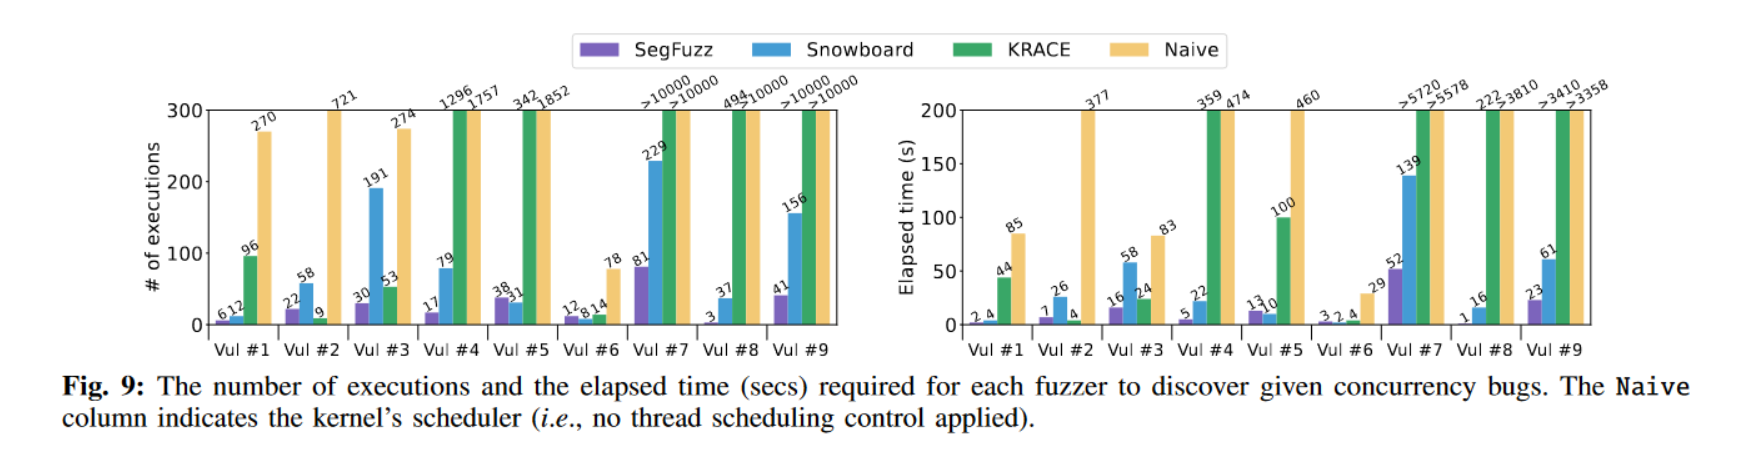
\includegraphics[width=0.8\linewidth]{fig13}
    \caption{\label{fig:fig13}每个模糊器发现给定并发错误所需的执行次数和所用时间(秒)。 Naive列指示内核的调度程序(未应用线程调度)。}
\end{figure}

总之,这些分析结果证实,即使交错段覆盖会构建比别名覆盖更复杂的搜索空间,基于突变的交错探索也通过快速导航搜索空间而表现出优越的性能。

\subsection{SEGFUZZ的性能特点}

本节提供了SEGFUZZ在覆盖范围增长、模糊测试吞吐量和每个输入开销方面的性能特征。

覆盖范围增长。由于覆盖率指标是模糊测试最重要的性能指标,因此我们测量了 100 小时模糊测试期间代码覆盖率(即采用的分支的数量)和交错覆盖率(即观察到的交错段的数量)的覆盖率增长。为了了解SEGFUZZ对线程交错探索的改进程度,我们在SEGFUZZ的多线程模糊测试阶段禁用线程调度控制(即随机线程调度),并测量交错覆盖率。图 11通过没有调度控制的交错段表示的行进行了描述。在禁用线程调度控制的情况下, SEGFUZZ发现同一时间段内交错段覆盖率减少了29.1\% 。为了确认这种改进来自实际的性能优势,我们在 24 小时内重复相同的实验,并使用 Mann-Whitney U 检验测量 p 值。p 值为 0.03,低于传统阈值0.05,表明观察到的改进可能是由SEGFUZZ的性能优势而不是随机性引起的。因此,我们可以得出结论,我们的设计选择在探索线程交错方面显著改进。


\begingroup
    \linespreadsingle{}
    \printbibliography[title={外文翻译参考文献}]
\endgroup
